% Options for packages loaded elsewhere
\PassOptionsToPackage{unicode}{hyperref}
\PassOptionsToPackage{hyphens}{url}
%
\documentclass[
  man,floatsintext]{apa6}
\usepackage{amsmath,amssymb}
\usepackage{iftex}
\ifPDFTeX
  \usepackage[T1]{fontenc}
  \usepackage[utf8]{inputenc}
  \usepackage{textcomp} % provide euro and other symbols
\else % if luatex or xetex
  \usepackage{unicode-math} % this also loads fontspec
  \defaultfontfeatures{Scale=MatchLowercase}
  \defaultfontfeatures[\rmfamily]{Ligatures=TeX,Scale=1}
\fi
\usepackage{lmodern}
\ifPDFTeX\else
  % xetex/luatex font selection
\fi
% Use upquote if available, for straight quotes in verbatim environments
\IfFileExists{upquote.sty}{\usepackage{upquote}}{}
\IfFileExists{microtype.sty}{% use microtype if available
  \usepackage[]{microtype}
  \UseMicrotypeSet[protrusion]{basicmath} % disable protrusion for tt fonts
}{}
\makeatletter
\@ifundefined{KOMAClassName}{% if non-KOMA class
  \IfFileExists{parskip.sty}{%
    \usepackage{parskip}
  }{% else
    \setlength{\parindent}{0pt}
    \setlength{\parskip}{6pt plus 2pt minus 1pt}}
}{% if KOMA class
  \KOMAoptions{parskip=half}}
\makeatother
\usepackage{xcolor}
\usepackage{graphicx}
\makeatletter
\def\maxwidth{\ifdim\Gin@nat@width>\linewidth\linewidth\else\Gin@nat@width\fi}
\def\maxheight{\ifdim\Gin@nat@height>\textheight\textheight\else\Gin@nat@height\fi}
\makeatother
% Scale images if necessary, so that they will not overflow the page
% margins by default, and it is still possible to overwrite the defaults
% using explicit options in \includegraphics[width, height, ...]{}
\setkeys{Gin}{width=\maxwidth,height=\maxheight,keepaspectratio}
% Set default figure placement to htbp
\makeatletter
\def\fps@figure{htbp}
\makeatother
\setlength{\emergencystretch}{3em} % prevent overfull lines
\providecommand{\tightlist}{%
  \setlength{\itemsep}{0pt}\setlength{\parskip}{0pt}}
\setcounter{secnumdepth}{-\maxdimen} % remove section numbering
% Make \paragraph and \subparagraph free-standing
\ifx\paragraph\undefined\else
  \let\oldparagraph\paragraph
  \renewcommand{\paragraph}[1]{\oldparagraph{#1}\mbox{}}
\fi
\ifx\subparagraph\undefined\else
  \let\oldsubparagraph\subparagraph
  \renewcommand{\subparagraph}[1]{\oldsubparagraph{#1}\mbox{}}
\fi
% definitions for citeproc citations
\NewDocumentCommand\citeproctext{}{}
\NewDocumentCommand\citeproc{mm}{%
  \begingroup\def\citeproctext{#2}\cite{#1}\endgroup}
\makeatletter
 % allow citations to break across lines
 \let\@cite@ofmt\@firstofone
 % avoid brackets around text for \cite:
 \def\@biblabel#1{}
 \def\@cite#1#2{{#1\if@tempswa , #2\fi}}
\makeatother
\newlength{\cslhangindent}
\setlength{\cslhangindent}{1.5em}
\newlength{\csllabelwidth}
\setlength{\csllabelwidth}{3em}
\newenvironment{CSLReferences}[2] % #1 hanging-indent, #2 entry-spacing
 {\begin{list}{}{%
  \setlength{\itemindent}{0pt}
  \setlength{\leftmargin}{0pt}
  \setlength{\parsep}{0pt}
  % turn on hanging indent if param 1 is 1
  \ifodd #1
   \setlength{\leftmargin}{\cslhangindent}
   \setlength{\itemindent}{-1\cslhangindent}
  \fi
  % set entry spacing
  \setlength{\itemsep}{#2\baselineskip}}}
 {\end{list}}
\usepackage{calc}
\newcommand{\CSLBlock}[1]{\hfill\break\parbox[t]{\linewidth}{\strut\ignorespaces#1\strut}}
\newcommand{\CSLLeftMargin}[1]{\parbox[t]{\csllabelwidth}{\strut#1\strut}}
\newcommand{\CSLRightInline}[1]{\parbox[t]{\linewidth - \csllabelwidth}{\strut#1\strut}}
\newcommand{\CSLIndent}[1]{\hspace{\cslhangindent}#1}
\ifLuaTeX
\usepackage[bidi=basic]{babel}
\else
\usepackage[bidi=default]{babel}
\fi
\babelprovide[main,import]{english}
% get rid of language-specific shorthands (see #6817):
\let\LanguageShortHands\languageshorthands
\def\languageshorthands#1{}
% Manuscript styling
\usepackage{upgreek}
\captionsetup{font=singlespacing,justification=justified}

% Table formatting
\usepackage{longtable}
\usepackage{lscape}
% \usepackage[counterclockwise]{rotating}   % Landscape page setup for large tables
\usepackage{multirow}		% Table styling
\usepackage{tabularx}		% Control Column width
\usepackage[flushleft]{threeparttable}	% Allows for three part tables with a specified notes section
\usepackage{threeparttablex}            % Lets threeparttable work with longtable

% Create new environments so endfloat can handle them
% \newenvironment{ltable}
%   {\begin{landscape}\centering\begin{threeparttable}}
%   {\end{threeparttable}\end{landscape}}
\newenvironment{lltable}{\begin{landscape}\centering\begin{ThreePartTable}}{\end{ThreePartTable}\end{landscape}}

% Enables adjusting longtable caption width to table width
% Solution found at http://golatex.de/longtable-mit-caption-so-breit-wie-die-tabelle-t15767.html
\makeatletter
\newcommand\LastLTentrywidth{1em}
\newlength\longtablewidth
\setlength{\longtablewidth}{1in}
\newcommand{\getlongtablewidth}{\begingroup \ifcsname LT@\roman{LT@tables}\endcsname \global\longtablewidth=0pt \renewcommand{\LT@entry}[2]{\global\advance\longtablewidth by ##2\relax\gdef\LastLTentrywidth{##2}}\@nameuse{LT@\roman{LT@tables}} \fi \endgroup}

% \setlength{\parindent}{0.5in}
% \setlength{\parskip}{0pt plus 0pt minus 0pt}

% Overwrite redefinition of paragraph and subparagraph by the default LaTeX template
% See https://github.com/crsh/papaja/issues/292
\makeatletter
\renewcommand{\paragraph}{\@startsection{paragraph}{4}{\parindent}%
  {0\baselineskip \@plus 0.2ex \@minus 0.2ex}%
  {-1em}%
  {\normalfont\normalsize\bfseries\itshape\typesectitle}}

\renewcommand{\subparagraph}[1]{\@startsection{subparagraph}{5}{1em}%
  {0\baselineskip \@plus 0.2ex \@minus 0.2ex}%
  {-\z@\relax}%
  {\normalfont\normalsize\itshape\hspace{\parindent}{#1}\textit{\addperi}}{\relax}}
\makeatother

\makeatletter
\usepackage{etoolbox}
\patchcmd{\maketitle}
  {\section{\normalfont\normalsize\abstractname}}
  {\section*{\normalfont\normalsize\abstractname}}
  {}{\typeout{Failed to patch abstract.}}
\patchcmd{\maketitle}
  {\section{\protect\normalfont{\@title}}}
  {\section*{\protect\normalfont{\@title}}}
  {}{\typeout{Failed to patch title.}}
\makeatother

\usepackage{xpatch}
\makeatletter
\xapptocmd\appendix
  {\xapptocmd\section
    {\addcontentsline{toc}{section}{\appendixname\ifoneappendix\else~\theappendix\fi: #1}}
    {}{\InnerPatchFailed}%
  }
{}{\PatchFailed}
\makeatother
\keywords{keywords\newline\indent Word count: X}
\usepackage{lineno}

\linenumbers
\usepackage{csquotes}
\ifLuaTeX
  \usepackage{selnolig}  % disable illegal ligatures
\fi
\usepackage{bookmark}
\IfFileExists{xurl.sty}{\usepackage{xurl}}{} % add URL line breaks if available
\urlstyle{same}
\hypersetup{
  pdftitle={How do different visual formats affect accuracy and reaction time in proportional reasoning tasks?},
  pdfauthor={Jennifer Curi1},
  pdflang={en-EN},
  pdfkeywords={keywords},
  hidelinks,
  pdfcreator={LaTeX via pandoc}}

\title{How do different visual formats affect accuracy and reaction time in proportional reasoning tasks?}
\author{Jennifer Curi\textsuperscript{1}}
\date{}


\shorttitle{Proportional Reasoning Across Formats}

\authornote{

Correspondence concerning this article should be addressed to Jennifer Curi. E-mail: \href{mailto:jdc294@rutgers.edu}{\nolinkurl{jdc294@rutgers.edu}}

}

\affiliation{\vspace{0.5cm}\textsuperscript{1} Rutgers University}

\abstract{%
This study looks at how people compare proportions shown in different ways, like dots or blobs. We checked if these formats change how accurate or fast people are. The results show that some formats make it easier to compare proportions, and taking more time can improve accuracy. These findings help us understand how the way information is shown affects how people think.
}



\begin{document}
\maketitle

\section{Introduction}\label{introduction}

Comparing proportions is sometimes very hard! But, even infants seem to be able to do it a little bit. The purpose of this science project was better understand how well people compare proportions when the proportions are presented in different formats. The purpose of this class assignment is to take the R-code and plots we've been generation over the last several weeks and put it all together into poster formal.

\subsection{Research Objectives}\label{research-objectives}

\begin{enumerate}
\def\labelenumi{\arabic{enumi}.}
\tightlist
\item
  Does average performance vary across format type?
\item
  Does average performance vary across numerator congruency
  status?
\item
  Does numerator congruency vary across format type? (i.e., is
  there an interaction)
\end{enumerate}

\section{Methods}\label{methods}

\subsection{Participants}\label{participants}

A total of 99 adults participated in the study.

First, participants were introduced to a story about a magic ball and that the outcome (i.e, blue or orange) depended on the proportions. They were then asked to compare the proportions of different images.

In other words, participants were shown two images of the same kind at the same time and asked to decide which had a higher proportion of the shape (or dots) colored in blue.

\begin{figure}
\centering
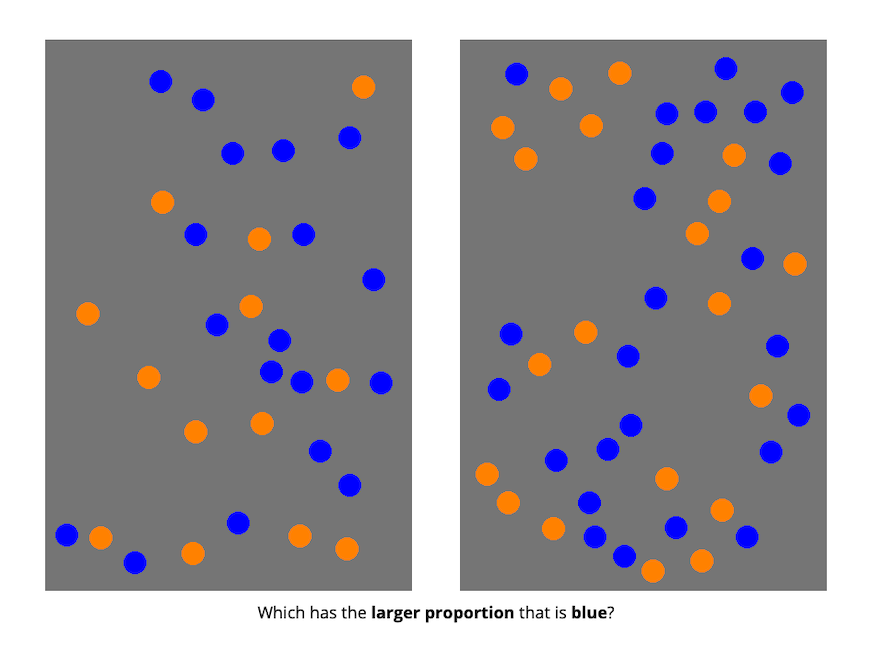
\includegraphics{images_WA10/Probtask_Trial.png}
\caption{\label{fig:graphicone}Results of visual stimuli used in the experiment.}
\end{figure}

\newpage

\subsection{Conditions}\label{conditions}

There were four different conditions that changed what kinds of
images the participants saw:

• divided blobs: blue and orange were entirely separate

• integrated blob: one blob, divided to be part blue and part orange

• separated dots: blue and orange dots were on opposite sides of
the image

• integrated dots: blue and orange dots were intermixed

\begin{figure}
\centering
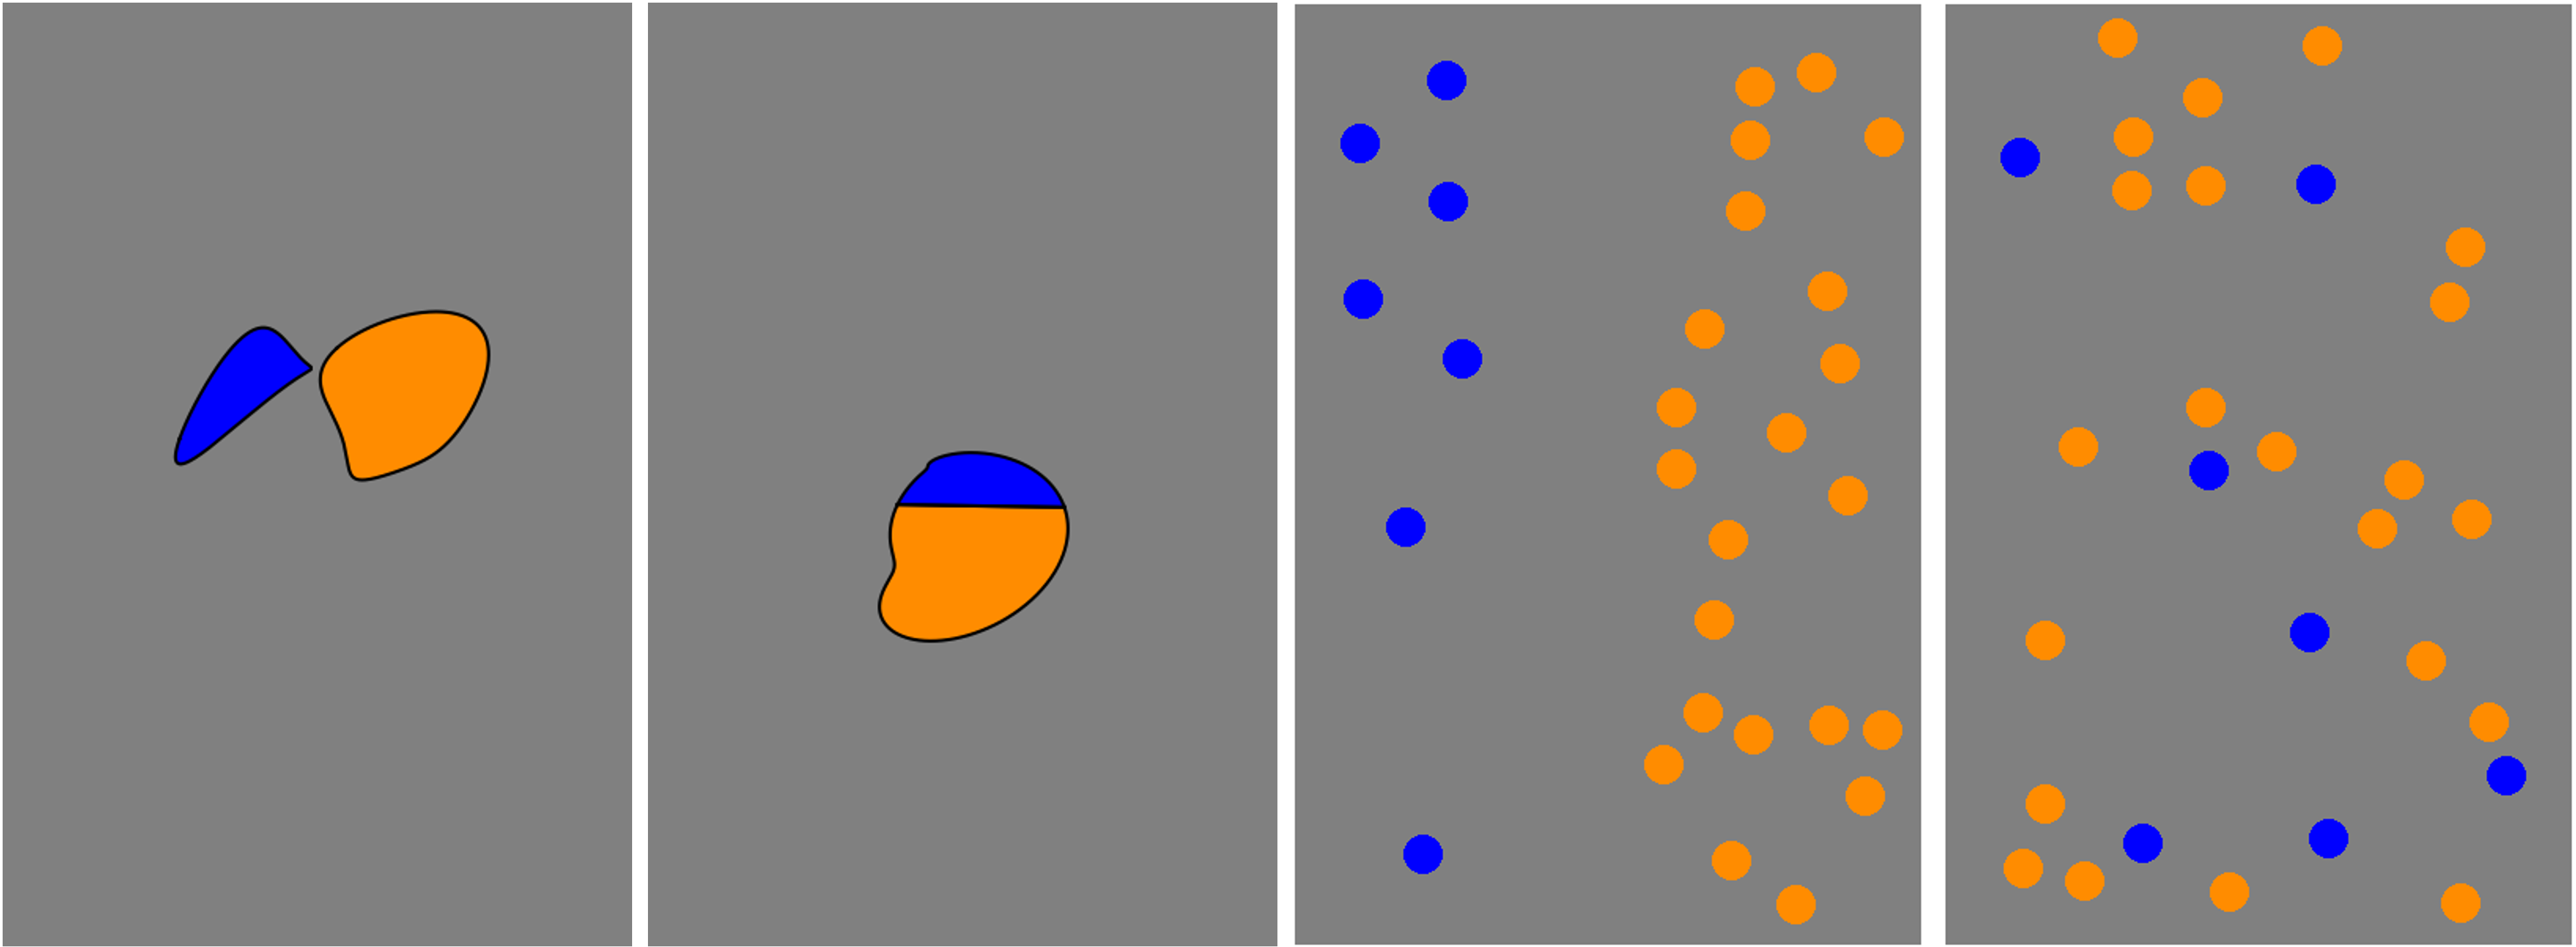
\includegraphics{../Assignment10/images_WA10/Probtask_formats.png}
\caption{\label{fig:graphictwo}Types of conditions.}
\end{figure}

\newpage

\section{Results}\label{results}

\begin{enumerate}
\def\labelenumi{\arabic{enumi}.}
\tightlist
\item
  Does average performance vary across format type, ignoring all other aspects of the stimuli?
\end{enumerate}

\begin{figure}
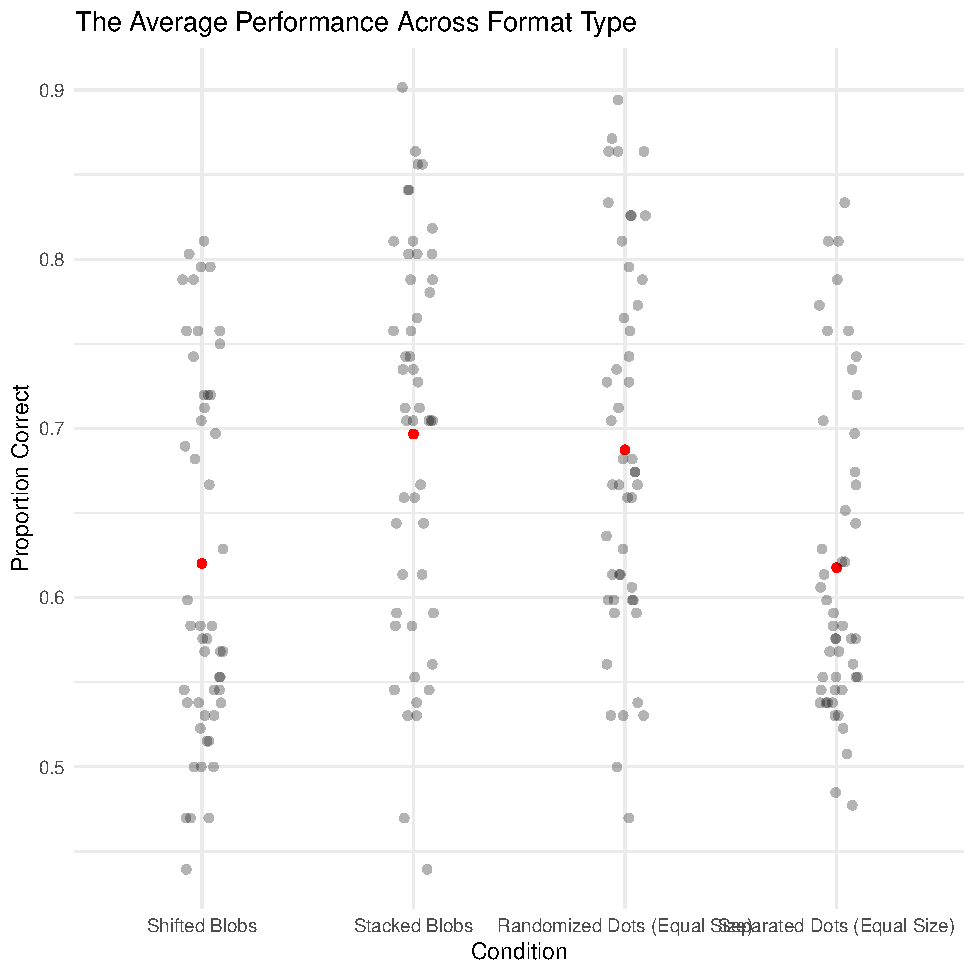
\includegraphics[width=0.8\linewidth]{Curi_11_files/figure-latex/plotone-1} \caption{The plot shows the average performance for each condition with red dots, while grey dots show how individual responses are distributed around these averages. The average accuracy (proportion correct), varies slightly across different format conditions}\label{fig:plotone}
\end{figure}

\newpage

\begin{enumerate}
\def\labelenumi{\arabic{enumi}.}
\setcounter{enumi}{1}
\tightlist
\item
  How are reaction time and accuracy related?

  \begin{figure}
  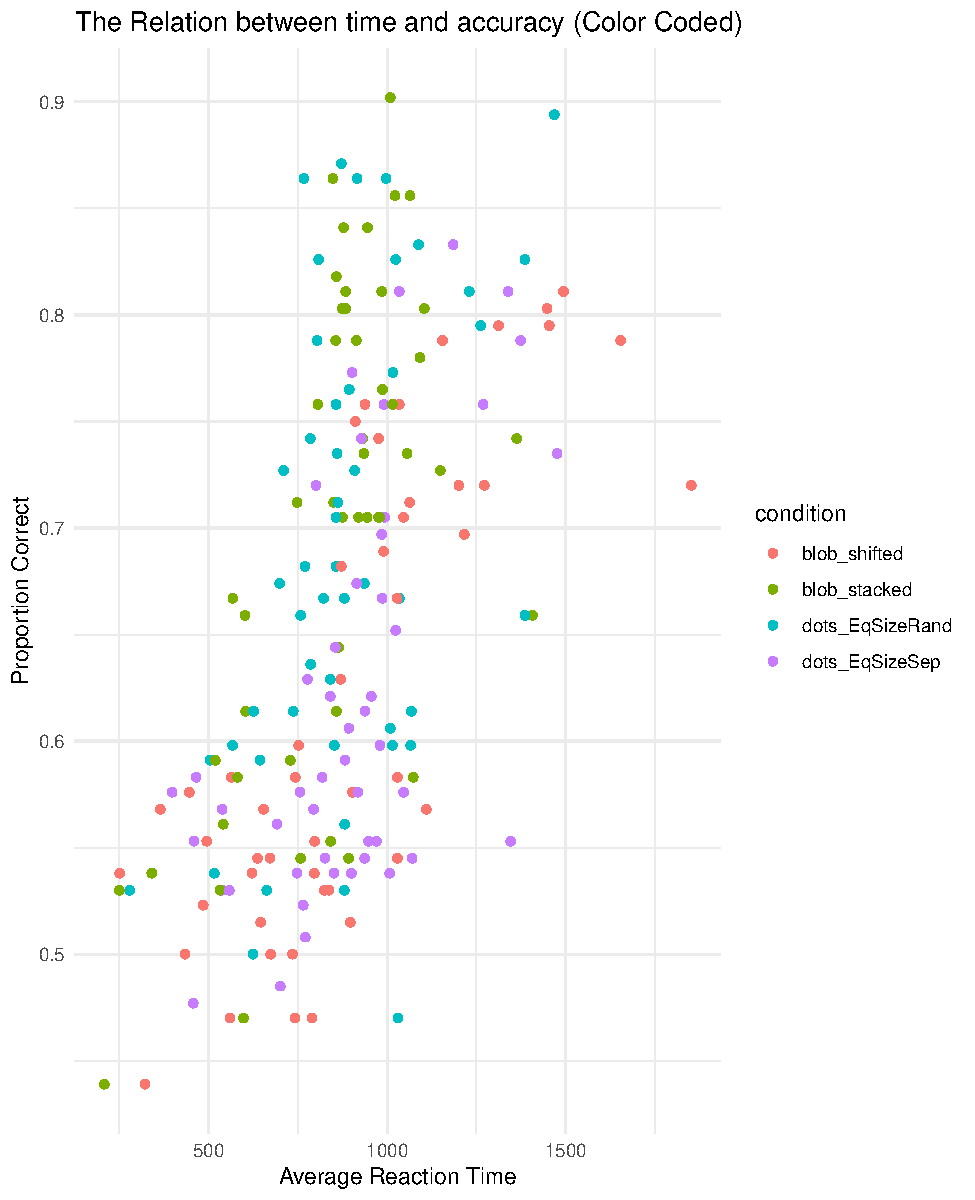
\includegraphics[width=0.7\linewidth]{Curi_11_files/figure-latex/plottwo-1} \caption{The plot shows that people tend to be more accurate when they take longer to respond, with different colors showing the results for each condition.}\label{fig:plottwo}
  \end{figure}
  \newpage
\item
  How does numerator congruency interact with format type?

  \begin{figure}
  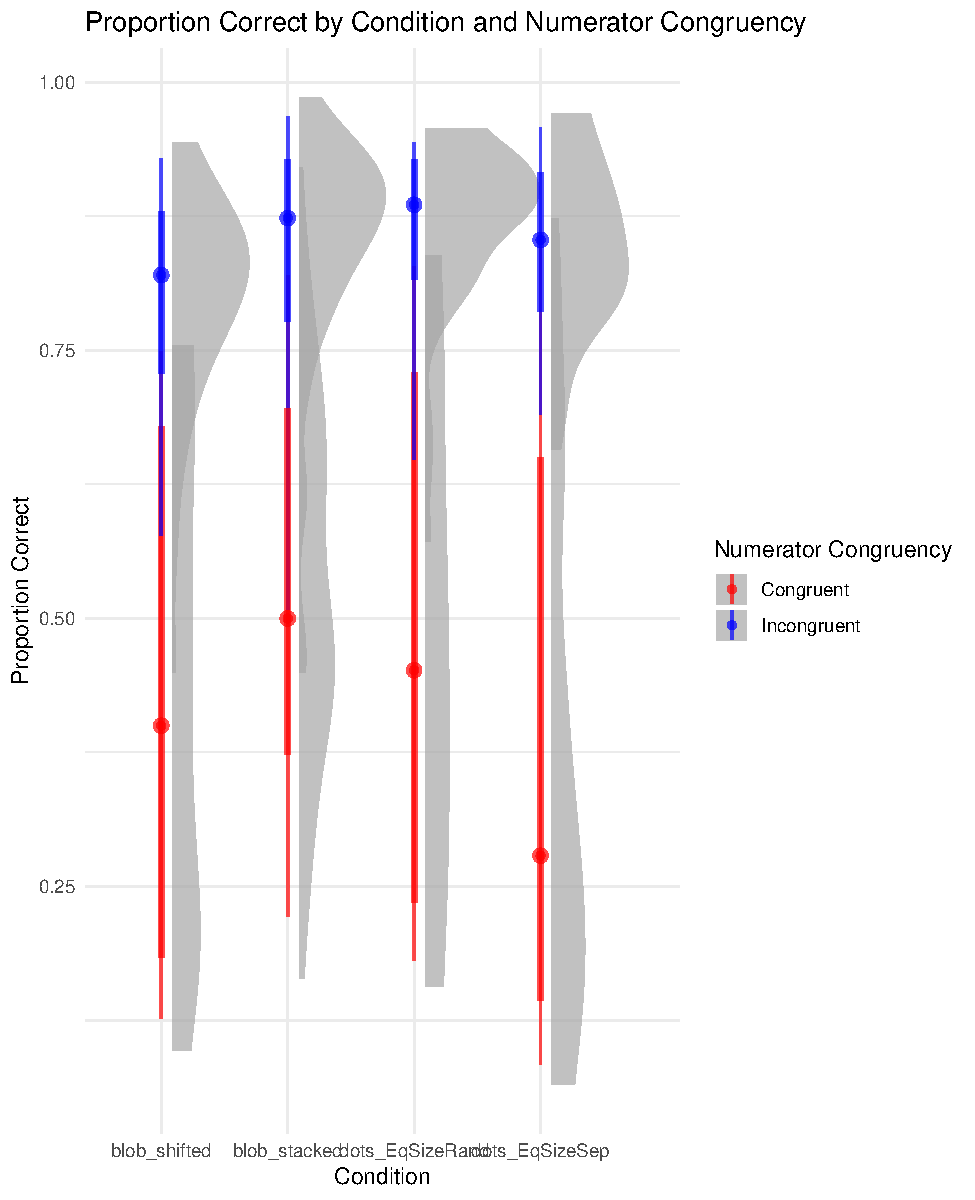
\includegraphics[width=0.7\linewidth]{Curi_11_files/figure-latex/plotthree-1} \caption{The plot shows that people tend to be less accurate on congruent trials (red) compared to incongruent trials (blue), and the performance varies across different conditions.}\label{fig:plotthree}
  \end{figure}
\end{enumerate}

\newpage

\section{Discussion}\label{discussion}

\subsection{Interpretation}\label{interpretation}

\textbf{Average Performance across format type:} The red dots show the average performance for each condition, while the grey dots show how individual responses vary. Some conditions have responses that are close to the average, while others show more spread, meaning participants' performance was less consistent.

\textbf{The Correlation between reaction time and accuracy:} This plot shows that people are usually more accurate when they take longer to respond. The different colors represent different conditions, and while the trend generally shows better accuracy with more time, there is still some variation between the conditions.

\textbf{How numerator congruency interacts with format types:} The plot compares performance on red (congruent) and blue (incongruent) trials. People tend to be less accurate on red trials compared to blue ones. The shaded areas show how much responses vary within each condition, with some conditions showing more spread than others.

\newpage

\subsection{Conclusion}\label{conclusion}

The tedious part of the assignment was dealing with the formatting and getting everything to look right on the poster. It took a lot of time to make sure each section was in the correct place and that the plots were accurate and displayed clearly. Because this was a new file, I had to re-summarize the prodtask data set and then graph it, which introduced some errors.

The most satisfying part was having a template to guide me, so I didn't have to start from 0. It saved me time and made it easier to focus on putting the content together. It also felt great to see all my work come together in the end. Seeing the finished poster with everything in place was rewarding and gave me a sense of accomplishment.

\newpage

\subsection{Data analysis}\label{data-analysis}

We used R (Version 4.3.0; R Core Team, 2023) and the R-packages \emph{dplyr} (Version 1.1.4; Wickham, François, Henry, Müller, \& Vaughan, 2023), \emph{forcats} (Version 1.0.0; Wickham, 2023a), \emph{ggdist} (Version 3.3.2; Kay, 2024), \emph{ggplot2} (Version 3.5.1; Wickham, 2016), \emph{lubridate} (Version 1.9.3; Grolemund \& Wickham, 2011), \emph{papaja} (Version 0.1.3; Aust \& Barth, 2024), \emph{purrr} (Version 1.0.2; Wickham \& Henry, 2023), \emph{readr} (Version 2.1.5; Wickham, Hester, \& Bryan, 2024), \emph{stringr} (Version 1.5.1; Wickham, 2023b), \emph{tibble} (Version 3.2.1; Müller \& Wickham, 2023), \emph{tidyr} (Version 1.3.1; Wickham, Vaughan, \& Girlich, 2024), \emph{tidyverse} (Version 2.0.0; Wickham, 2023c) and \emph{tinylabels} (Version 0.2.4; Barth, 2023) for all our analyses.

\newpage

\phantomsection\label{refs}
\begin{CSLReferences}{1}{0}
\bibitem[\citeproctext]{ref-R-papaja}
Aust, F., \& Barth, M. (2024). \emph{Papaja: Prepare american psychological association journal articles with r markdown}. Retrieved from \url{https://github.com/crsh/papaja}

\bibitem[\citeproctext]{ref-R-tinylabels}
Barth, M. (2023). \emph{{tinylabels}: Lightweight variable labels}. Retrieved from \url{https://cran.r-project.org/package=tinylabels}

\bibitem[\citeproctext]{ref-R-lubridate}
Grolemund, G., \& Wickham, H. (2011). Dates and times made easy with {lubridate}. \emph{Journal of Statistical Software}, \emph{40}(3), 1--25. Retrieved from \url{https://www.jstatsoft.org/v40/i03/}

\bibitem[\citeproctext]{ref-R-ggdist}
Kay, M. (2024). \emph{Ggdist: Visualizations of distributions and uncertainty}. Retrieved from \url{https://mjskay.github.io/ggdist/}

\bibitem[\citeproctext]{ref-R-tibble}
Müller, K., \& Wickham, H. (2023). \emph{Tibble: Simple data frames}. Retrieved from \url{https://CRAN.R-project.org/package=tibble}

\bibitem[\citeproctext]{ref-R-base}
R Core Team. (2023). \emph{R: A language and environment for statistical computing}. Vienna, Austria: R Foundation for Statistical Computing. Retrieved from \url{https://www.R-project.org/}

\bibitem[\citeproctext]{ref-R-ggplot2}
Wickham, H. (2016). \emph{ggplot2: Elegant graphics for data analysis}. Springer-Verlag New York. Retrieved from \url{https://ggplot2.tidyverse.org}

\bibitem[\citeproctext]{ref-R-forcats}
Wickham, H. (2023a). \emph{Forcats: Tools for working with categorical variables (factors)}. Retrieved from \url{https://CRAN.R-project.org/package=forcats}

\bibitem[\citeproctext]{ref-R-stringr}
Wickham, H. (2023b). \emph{Stringr: Simple, consistent wrappers for common string operations}. Retrieved from \url{https://CRAN.R-project.org/package=stringr}

\bibitem[\citeproctext]{ref-R-tidyverse}
Wickham, H. (2023c). \emph{Tidyverse: Easily install and load the tidyverse}. Retrieved from \url{https://tidyverse.tidyverse.org}

\bibitem[\citeproctext]{ref-R-dplyr}
Wickham, H., François, R., Henry, L., Müller, K., \& Vaughan, D. (2023). \emph{Dplyr: A grammar of data manipulation}. Retrieved from \url{https://CRAN.R-project.org/package=dplyr}

\bibitem[\citeproctext]{ref-R-purrr}
Wickham, H., \& Henry, L. (2023). \emph{Purrr: Functional programming tools}. Retrieved from \url{https://CRAN.R-project.org/package=purrr}

\bibitem[\citeproctext]{ref-R-readr}
Wickham, H., Hester, J., \& Bryan, J. (2024). \emph{Readr: Read rectangular text data}. Retrieved from \url{https://CRAN.R-project.org/package=readr}

\bibitem[\citeproctext]{ref-R-tidyr}
Wickham, H., Vaughan, D., \& Girlich, M. (2024). \emph{Tidyr: Tidy messy data}. Retrieved from \url{https://CRAN.R-project.org/package=tidyr}

\end{CSLReferences}


\end{document}
